\documentclass[17pt]{extarticle}
\usepackage{amsmath, amssymb}
\usepackage{nccmath}
\usepackage[a4paper, total={6.5in, 9.5in},top=2mm,left=27mm]{geometry}
\usepackage{titlesec}
\usepackage{tikz}
\usepackage{gensymb}
\usetikzlibrary{arrows.meta}

\titleformat{\section}
{\normalfont\normalsize\bfseries}{\thesection}{1em}{}
\setcounter{secnumdepth}{0} %% no numbering for sections

\begin{document}
\noindent
\begin{fleqn} 

%%%%%%%%%%%%%%%%%%%%%%%%%%%%%%%%%%%%%%%%%%%%%%%%%%%%%%%%%%%%%%%%

\section{Question: 01}
A box is made with a square base and open top. The area of material for making the box is 300 sq. cm. Find the dimensions of the box, if its volume is maximum. Also find the maximum volume.

%----------------------------------------

\section{Answer: 01}
Let OA and OB be the lines passing through the origin making an angle of
 $ 60\degree$ with the line $y = 3.$ \\

\begin{equation} \nonumber
\begin{alignedat}{4}
& \therefore h = \frac{300 - x^2}{4x}\\
& \text{ Base Volume V} \\
&= \text{Area of Base x Height}\\
&= x^2\left(\frac{300-x^2}{4x}\right)\\
&= \frac{1}{4}(300x - x^2)
\end{alignedat}
%\vrule
\quad\quad\quad
\begin{alignedat}{4}
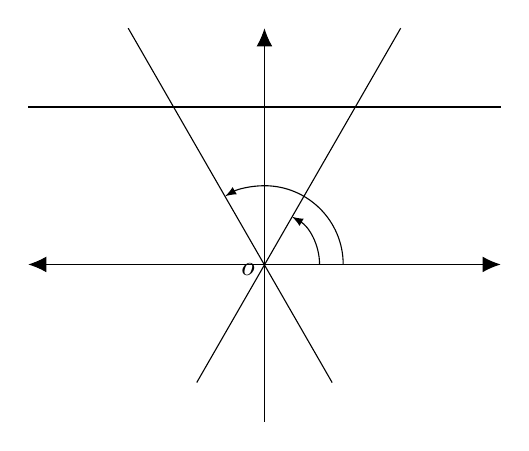
\begin{tikzpicture}
\draw [>={LaTeX[width=2mm,length=2.3mm]},<->](-3,0) -- (3,0);
\draw [>={LaTeX[width=2mm,length=2.3mm]},->](0,-2)  -- (0,3);
\draw (-3,2) -- (3,2);
\draw (-0.86,-1.5) -- (1.73,3);
\draw (-1.73,3) -- (0.86,-1.5);
\draw (0,0) node[anchor=north east,yshift=4pt] {$o$} ;
%\filldraw[fill=green!20,draw=green!50!black] (0,0) -- (0.7,0) arc (0:60:0.7) -- cycle;

\draw[-latex] (0:0.7cm) arc (0:60:0.7cm);
%\draw (0,0)  -- (1,0) arc (0:120:1) -- cycle;
\draw[-latex] (0:1cm) arc (0:120:1cm);
\end{tikzpicture}
\end{alignedat}
\end{equation}
\quad


\begin{equation} \nonumber
\begin{alignedat}{4}
& \frac{dV}{dx}=\frac{1}{4}(300x - x^2) \\
& But\  \frac{dV}{dx}= 0 \text{ for max}\\
& \therefore \frac{1}{4}(300x - x^2)=0\\
& \therefore x = \pm 10\\
& \therefore x = 10 \ \ (+ve)
\end{alignedat}
\quad
\vrule
\quad
\begin{alignedat}{4}
&= \left(\frac{d^2V}{dx^2}\right)_{x=10}=\left(\frac{-3x}{2}\right)_{x=10} = -15<0\\
& \therefore \text{ V is max at x = 10 by 2nd derivative test}\\
& \therefore Height\  h=But\  \frac{300 - (10)^2}{4(10)}= 5\ cm\\
& \therefore Required\  dim = 5 \times  5 \times 10 \\
& Consequently \ Volume\ V = 500 \ cm^3 \\
\end{alignedat}
\end{equation}

%%%%%%%%%%%%%%%%%%%%%%%%%%%%%%%%%%%%%%%%%%%%%%%%%%%%%%%%%%%%%%%%%%%%%%%%%%

\end{fleqn}
\end{document} 